\chapter{Introduction}

Microservices have emerged in the last decade as a approach for architecting and organising software as a fleet of autonomous and specialised services, that are loosely-coupled, easier to develop and maintain compared to traditional monolithic architectures. Automated and independent deployment, focus on business capabilities, communication via well-defined interfaces using lightweight APIs, decentralised governance and data management are commonly observed characteristics of this evolving architectural style.

\begin{figure}[ht]
  \centering
  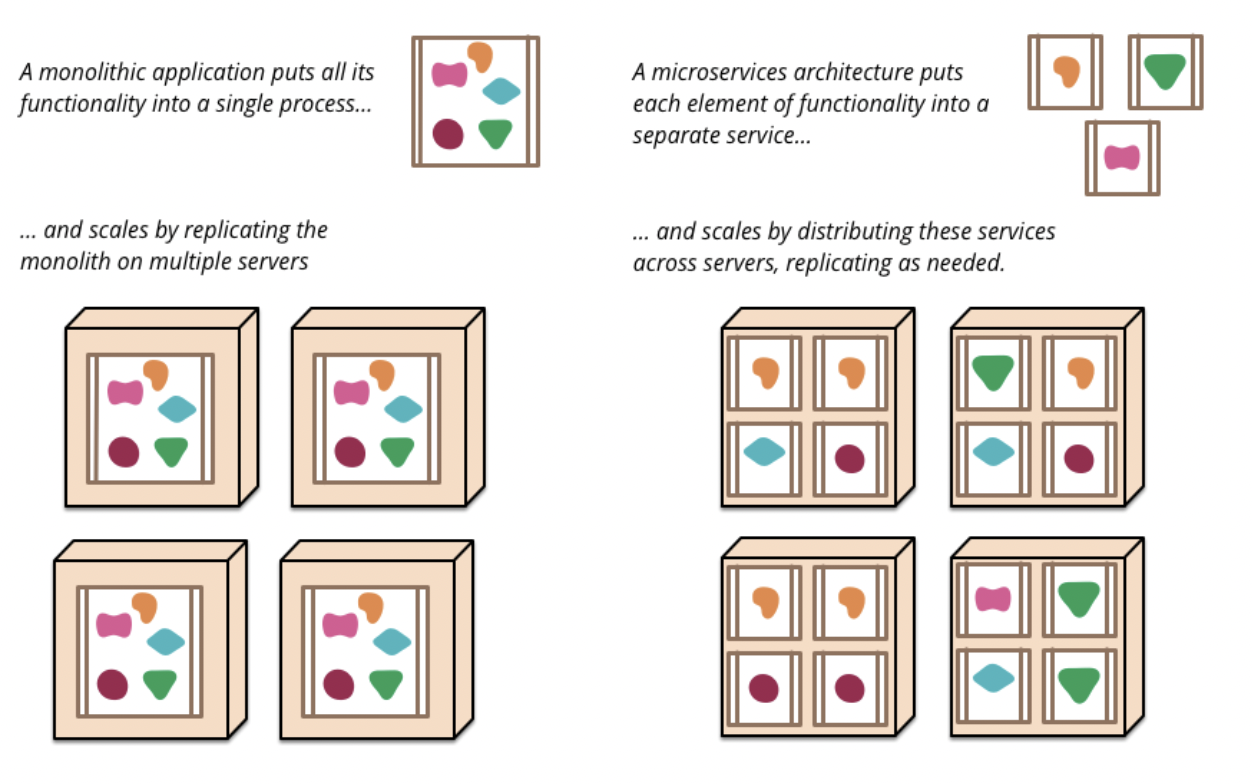
\includegraphics[width=0.65\linewidth]{./assets/images/mono-micro-lewis.png}
  \caption{Monoliths versus microservices \cite{lewis14}.}
  \label{fig:mono-micro-lewis}
\end{figure}

Design patterns in software engineering are well-documented templates describing common problems and recommended approaches in a given context. For nearly 30 years, design patterns and anti-patterns have guided developers to build software systems without having to re-invent the wheel every step of the way. As microservices haven't reached full maturity yet, system design choices guided by appropriate design pattern choices have a massive impact on the functionality and performance of applications. Performance engineering is an often ignored aspect of software design, but is in fact vital to its overall success, especially with the growth of business and changing demands. It encompasses performance analysis at design and deployment time, as well as performance monitoring and management at run-time. Although microservices have seen several stages of evolution over the years, innovation has been driven primarily by leading companies in the software industry, without significant contribution from academia. The motivation for conducting this project is the lack of adequate studies on the effect of design pattern choices on the performance of microservice-based systems.

This project explores the performance implications of a number of design patterns implemented by two microservice-based web applications. The systems have been developed to model a movie ticket reservation systems, involving a client, three independent cinemas, and an intermediary service to handle client interactions. The first case study conducted explores patterns such as an API gateway, circuit breaker and service discovery. The second study's application implements patterns including asynchronous messaging, monitoring of application metrics and health check API. In addition, both studies demonstrate indispensable patterns such as externalised configuration, separate database per service, and deployment as service instance per container. In the end, the performance of systems is evaluated using both quantitative and qualitative metrics, allowing us draw some comparisons between two case studies.

